\chapter{Model Design and Implementation}
\label{chp:chapter3}
\graphicspath{{figures/}{figures/chapter3/}}

\section{Overview} \label{Overview}

The objective of this study is to evaluate the relative systemic
criticality of highway links on a statewide network using a logit-based model
sensitive to changes in route path, destination choice, and mode choice.

In this chapter, some of USTM's properties are described, and additional detail is give as to why
USTM is not entirely suitable for this study as presently constituted. A new model framework designed to evaluate resilience using a logit-based choice model on
USTM's network is then presented. Implementation of this new model within the CUBE travel demand
modeling software is also described.

\section{Utah Statewide Travel Model} \label{Utah Statewide Travel Model}

UDOT manages an extensive highway
network consisting of interstate highways (e.g., I-15, I-80, I-70, and I-84),
intraurban expressways along the Wasatch Front, and rural highways throughout
the state. The rugged mountain and canyon topography places
severe constraints on possible redundant paths in the highway network. A
landslide or rock fall in any single canyon may isolate a community or force a
redirection of traffic that could be several hours longer than the preferred
route; understanding which of these many possible choke points is most
critical is a key and ongoing objective of the agency.

USTM is developed and maintained by
the Travel Demand Modeling group at UDOT, and focuses exclusively on
long-distance trips. Within Utah, there are five travel
demand models developed for urban centers under the purview of  Metropolitan
Planning Organizations (MPOs). USTM incorporates these other models as inputs and covers
the rural areas lying outside of the MPO model regions. Consequently, USTM covers the
highway facilities across the entire state, and incorporates the MPO models
developed by the Wasatch Front Regional Council (WFRC), Mountainland
Association of Governments (MAG), Cache Metropolitan Planning Organization, and the Dixie Metropolitan Planning Organization. Additionally,
the Summit/Wasatch Travel Demand Model is incorporated into USTM \citep{udot2021}.
USTM as currently
constituted can be used for infrastructure planning purposes, but would be
inadequate to evaluate the systemic resiliency of the highway network given
the disparate methodologies of the MPO models incorporated. USTM can, however, provide the
following data elements:

\begin{description}
\def\labelenumi{\arabic{enumi}.}
\item
  {Highway Network}: including free flow and congested travel speeds,
  link length, link capacity estimates, etc.
\item
  {Zonal Productions}: available for all zones by purpose,
  including those in the MPO region areas
\item
  {Calibration Targets}: USTM base scenario estimates of mode split and
  trip length that could be used to calibrate the utility coefficients of a new model
\end{description}

Each of the local travel demand models and USTM employ a gravity-based trip
distribution model. The gravity model assumes that trips between OD
pairs are proportional to total productions $P$ and
attractions $A$ throughout the state. That is, all productions will be
attracted to a location based on the size of a location (i.e., a location's
attractiveness) and the impedance (or friction) factor between the OD
pair. A mathematical representation of the gravity model is given by:

\begin{equation}
T_{ij}= \frac{P_i*(A_j F_{ij})}{\sum_{j\in J}(A_j F_{ij})}
 \label{eqn:gravity}
\end{equation}

\noindent where $T_{ij}$ represents the trips made between an origin $i$ and a
  destination $j$ among all destinations $J$, $P_i$ represents the productions at origin $i$, $A_j$ represents the attractions and destination $j$, and $F_{ij}$ is the impedance factor between an $OD$ pair.
The friction factor (also known as the impedance, or resistance to movement) between two
zones can be represented in a number of ways, such as with a negative
exponential function:

\begin{equation}
	F_{ij} = \alpha \exp(-\beta * d_{ij})
  \label{eqn:fricfac}
\end{equation}

\noindent where $d_{ij}$ is the distance or cost between zones $i$ and $j$, and $\alpha$
and $\beta$ are calibrated parameters. In the gravity model, as the distance
between an OD pair increases, users become less likely to make trips between
that OD pair. Destinations are fixed, and trips calculated using the
gravity model must have a proportional number of users assigned to each
destination based on its size or level of attraction (i.e., in an ideal
scenario, if there are 100
productions, there should be 100 attractions).

A primary weakness of gravity-based distribution models is their inability to
consider multimodal impedances or other attributes of a destination other than
a destination's size (as represented by $A_j$ in Equation \ref{eqn:gravity}). The
impedance factor in Equation \ref{eqn:fricfac} asks an implicit question with its
distance or cost variable $d_{ij}$: which mode is used for the trip? In almost
all cases, automobile distances are asserted as the only option, but if a
destination happens to be close by rail and far by highway, the gravity model
will not be able to incorporate this unless a mode split function is carried out first.

Alternatively to gravity models, logit-based models are becoming
increasingly more popular for trip distribution. Logit-based destination choice models improve model
sensitivity compared with gravity models, and are advantageous because
they possess an increased ability to introduce additional variables and reflect
other statistical assumptions into a model \citep{tfr2021}. A typical choice
model is made up of a combination of utility and probability values in the
following equations:

\begin{equation}
\mathcal{P}_{ij} = \frac{e^{u_{ij}}}{\sum_{j\in J}e^{u_{ij}}}
  \label{eqn:probability}
\end{equation}

\noindent where $\mathcal{P}_{ij}$ represents the probability of trips made between an
origin \(i\) and a destination \(j\) among all destinations $J$, and \(u\) represents the utility. The probabilities
calculated are then used to calculate the mode or destination choice probability,
which allow trips by purpose and trips by mode to be calculated. These Equations
are shown in Equations \ref{eqn:ij} and \ref{eqn:ijk} later in this chapter. Then
we have the logsum calculation, which is the denominator of the probability function.
The logsum captures the total value of the choice set, and is interpreted as the
benefit --- or dis-benefit --- experienced by users in a choice model.

\begin{equation}
 Logsum_{i} = \ln\sum_{j\in J}\exp(f(\beta, u_{ij}, A_j, \gamma, t_{ij}))
  \label{eqn:logsum}
\end{equation}

\noindent where $\beta$ represents a mode choice coefficient, $u_{ij}$ represents the utility,
$A_j$ represents the attraction at zone $j$, $\gamma$ represents
a DC parameter, and $t_{ij}$ represents the travel time between an OD pair.

The ability to incorporate multiple types of data, as in Equation \ref{eqn:logsum}, as well as improved methods
for determining trip distribution, mode choice, and destination choice all allow
logit-based models to add an additional layer of sensitivity into estimations of
trips between OD pairs on a road network. Consequently, logit-based travel
demand models are better equipped to estimate the choice-based effects caused
by major changes to a road network, such as link loss or major link degradation
caused by adverse natural or man-made events.

Destination choice models explicitly consider multimodal accessibility, such as accessibility by automobile,
non-motorized trip, or transit. The ability to consider accessibility from a
multimodal perspective gives a user the ability to choose the location of
their destination based on a variety of factors including mode accessibility
(i.e. ease of access to a mode of transport). The information
derived from the socioeconomic data primarily comprises the size term, which
is a measure of the appeal or attractiveness of one destination when compared with
another destination. The DC size term is discussed in further detail in
Section \ref{sec:dc}.

A critical feature of logit-based choice models – described briefly in Section
\ref{sec:cacc} – is that they are more versatile than traditional modeling
methods, with the ability to incorporate different types of data --- \textit{and}
account for user choice. Additionally, logit-based choice models are better
able to measure the changes in accessibility of a destination due to network
changes than other models because of their adaptive nature. As such, logit-based
models are typically used in new or more advanced travel models.

Logit-based destination choice models are becoming increasingly common in four-
step and other modern travel models. However, no logit-based destination
choice models have been implemented within an MPO model in Utah or within
USTM except for some home-based work trips in the WFRC/MAG model. As a result,
the local MPO models, and therefore USTM, are not sufficient to analyze
accessibility on their own as proposed by this thesis. Therefore, a new
standalone model must be developed to examine choice-based resiliency in Utah.

\section{Model Design} \label{Model Design}

An initial model framework was developed to ensure a robust logit-based model
could be created. The model framework used to create the Resiliency Model
consists of the following steps:

\begin{description}
	\item {Skim Network} - In this step, the model determines the shortest
  path by AM peak travel time on the USTM network between each origin and
  destination. The model also determines the distance of the shortest time
  path. Transit times are given by an external data source.
	\item {Mode Choice Logsum} - The mode choice logsum is a function of
  the travel impedances and serves as an accessibility term in the destination
  choice model. The mode choice logsum contains utility functions that
  determine the probability and logsum associated with travel between each OD
  pair. The mode choice model also contains constants and coefficients that can
  be used to calibrate and adjust the utility equations, determining the mode
  choice probabilities.
	\item {Destination Choice (DC) Logsum} - The destination choice logsum
  is a function of the travel impedances (represented by the mode choice logsum)
  and the attraction size term of each destination zone. This is the key
  evaluation metric of the model because of the ability to incorporate multiple
  data types into the model structure. The attraction size term is determined
  using socioeconomic data for each destination zone given by USTM.
\end{description}

  \begin{figure}
    \centering
  {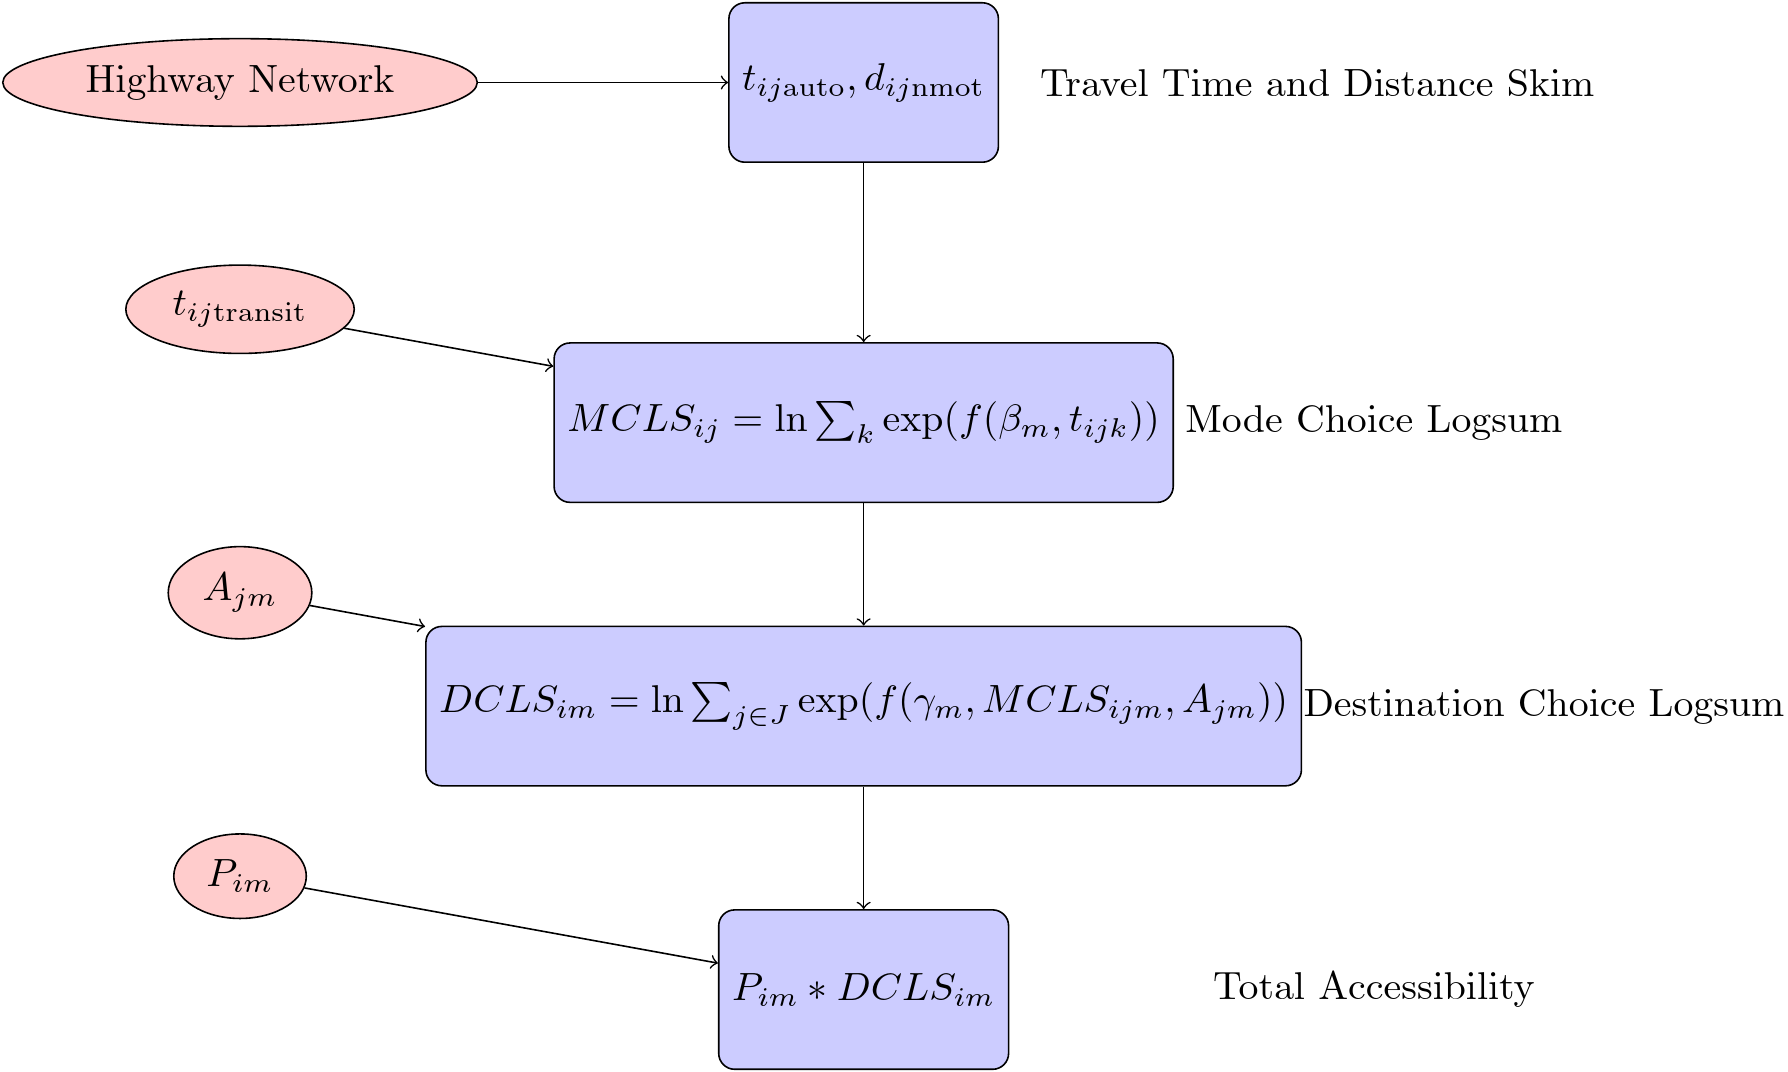
\includegraphics[width=0.75\linewidth]{figures/chapter3/framework.png}}
  \caption{Resiliency Model framework.}\label{fig:framework}

  \end{figure}

The model framework as used is presented in Figure \ref{fig:framework}, where
inputs are denoted with red ovals, and functions are denoted with purple rectangles.
The model framework is designed to capture the utility-based accessibility for
a particular origin zone \(i\) and trip purpose \(m\). The model begins with a
travel time skim procedure, to determine the congested travel time from zone
\(i\) to zone \(j\) by auto (i.e., \(t_{ijdrive}\)), as well as the shortest network distance (i.e., \(d_{ijnmot}\)) for non
motorized modes using the USTM network. The transit travel time skim is fixed, assuming that transit
infrastructure would not be affected by changes to the highway network, thus \(t_{ijtransit}\) is held fixed.
Throughout this section, acronyms from the model framework will be described and lower-cased index variables \(k\) belong to a set of
all indices described by the corresponding capital letter \(K\).

With the travel time \(t_{ijk}\) and distance for all modes \(k \in K\), the
model computes mode choice utility values. The multinomial logit mode choice
model describes the probability of a person at origin \(i\) choosing mode \(k\)
for a trip to destination \(j\):

\begin{equation}
\mathcal{P}_{ijm}(k) = \frac{\exp(f(\beta_m * t_{ijk}))}
{\sum_{K}\exp(f(\beta_m * t_{ijk}))}
  \label{eq:mcp}
\end{equation}

\noindent The log of the denominator of the this equation is called the
mode choice logsum, \(MCLS_{ijm}\) or \(MCLS\) and is a measure of the travel cost by
all modes, $k$, weighted by MC utility parameters \(\beta\) that may vary by
trip purpose $m$. The parameter values are described in greater detail in
Table \ref{tab:coeffs}.

The \(MCLS\) is then used as a travel impedance term in the multinomial
logit
destination choice model, where the probability of a person at origin \(i\)
choosing destination \(j \in J\) is

\begin{equation}
\mathcal{P}_{im}(j) = \frac{\exp(f(\gamma_m, MCLS_{ijm}, A_{jm}))}
{\sum_{J}\exp(f(\gamma, MCLS_{ijm}, A_j))}
  \label{eq:dcp}
\end{equation}

\noindent where \(A_j\) is the attractiveness --- represented in terms of
socioeconomic activity --- of zone \(j\). As with mode choice, the log of the
denominator of this model is the
destination choice logsum, \(DCLS_{im}\) or \(DCLS\). This quantity represents the value of access to
all destinations
by all modes of travel, and varies by trip purpose.

The \(DCLS\) measure is relative, but can be compared across
scenarios. The difference between the measures of two scenarios,

\begin{equation}
\Delta_{im} = {DCLS_{im}}^{\mathrm{Base}} - {DCLS_{im}}^{\mathrm{Scenario}}
  \label{eq:deltas}
\end{equation}

 \noindent provides an estimate of the accessibility lost when
 \(t_{ij\mathrm{auto}}\)
changes due to a damaged highway link. This accessibility change is \emph{per
trip},
meaning that the total lost accessibility is \(P_{im} * \Delta_{DCLS}\) where
\(P\) is
the number of trip productions at zone \(i\) for purpose \(k\). This measure is
given in units of dimensionless utility, but the mode choice cost coefficient
\(\beta\) provides a conversion factor between utility and cost. The total
financial
cost of a damaged link for the entire region for all trip purposes is:

\begin{equation}
\mathrm{Cost} = \sum_{I}\sum_{M} -1 / \beta_{\mathrm{cost},m} * P_{im}
\Delta_{im}
  \label{eq:totalcost}
\end{equation}

For comparison to a simpler resilience method that only includes the increased
travel time between an OD pair, we compute the change in travel
time, \(\Delta t_{ij}\), between two scenarios, and multiply the number of trips by this change
and a value of time coefficient derived from the cost and vehicle time
coefficients of the mode choice model,
\begin{equation}
\mathrm{Cost}' =  \sum_I \sum_J \sum_K \frac{\beta_{\mathrm{time}, k}
}{\beta_{\mathrm{cost}, k}} T_{{ijm}_{auto}} t_{{ij}_{auto}}
  \label{eq:ttmethod}
\end{equation}

\noindent Deriving a simpler way to calculate resilience was necessary for two
reasons. First, data were not readily available for trips that do not have
flexible OD pairs, such as freight trips. Other purposes included in USTM,
such as recreation trips (REC) and trips that occur between external nodes
(i.e., inter-state trips that do not originate or terminate within the state),
make up very small percentage of total trips. Second, a method capable of
creating data that could be compared with the results of the Resiliency Model
was needed. Calculating dis-benefit
based solely on increased travel time provides valuable insight and tools for
further analysis of the Resiliency Model results.

\section{Model Inputs}

MAX PUT A PARAGRAPH HERE

\subsection{Transportation Networks}

The Resiliency Model requires an understanding of the distance between zones by multiple modes, and how
these distances change when a link in the network is damaged or destroyed. To measure the
automobile, transit, and non-motorized trip times, initial data were needed for each trip mode.

The highway network is made up of both the urban and rural highway networks
for the whole state of Utah. The highway network contains many link- and
node-attribute data including street name, link distance, lanes, functional
classification, transportation analysis zone number (TAZ), county name,
as well as speed limits and travel time data for five different times of day.
Of particular interest from the available information was the \(AM\_TIME\) which
contains the travel time in minutes for the AM time period along a link and
the \(DISTANCE\), which contained the linear distance between nodes along a link.
The \(AM\_TIME\) was used to determine the travel time between an origin and
destination. The \(DISTANCE\) was used to measure the network distance between
the shortest OD pair based on AM travel time.

The highway skim module creates an output matrix (i.e., the highway skim) of travel
times and distances between OD pairs and must be created
before automobile (AUTO) and non-motorized (NMOT) trips can be incorporated
into the model. We used the \(AM\_TIME\) and \(DISTANCE\) variables available in
the highway network file to create a matrix of distances and shortest travel
times between all OD pairs in the USTM network. The output matrix forms the
basis for further analysis by providing the needed automobile and non-motorized
information for the other modules in the model.

Transit network resiliency is outside the scope of this project. Accordingly, the Resiliency
Model assumes that transit services are fixed, meaning that changes to the
network do not influence transit availability on the network. However, transit
is an important mode to include in the Resiliency Model, and  should be
considered in future model development if applicable for more robust analysis.
Among MPO models in Utah, only the model jointly operated by the WFRC and MAG model include a
substantive transit forecasting component. The transit travel time skim from the
WFRC/MAG model was used for the mode choice model in Equation \eqref{eq:mcp};
the zonal travel time between the smaller WFRC/MAG model zones was averaged
to the larger USTM zones using a crosswalk, or matrix transformation function, and the minimum time among the several modes available
(commuter rail, light rail, bus rapid transit, local bus) was taken as the travel
time for a single transit mode in this implementation.

The NMOT trip distances are held fixed, similarly to the transit distances. It was
determined that the longest distance a pedestrian would commute via a NMOT
mode is 2.5 miles or less. The decision to hold NMOT
trips constant was made for several reasons, mainly because pedestrians can usually
access routes that are not available to vehicles, such as neighborhood walkways/bikeways
or other shortcuts available only to pedestrians and cyclists. Additionally,
pedestrians are often also able to cut through or traverse the perimeter of an
area where a highway may be degraded or damaged. NMOT trips also typically have
higher accessibility to smaller roads or side-streets that would not be included
with the USTM network.

\subsection{Trip Productions and Socioeconomic Data}

The Resiliency Model uses socioeconomic data to estimate the productions at
each zone. The socioeconomic data, which is adapted from the UTS conducted in 2013, contains TAZ related information such
as county name, total households, household population, total employment,
and a breakdown of employment by job category, among other data. This information is useful
when determining the DC attractions, or size term because they can be used to
describe population density of residential zones, or business density and type
of commercial zones in a network. More importantly perhaps, is that the size
term denotes the significance of a TAZ in attracting trips. The size term is
created using various DC parameters combined with corresponding socioeconomic data
to determine the size or attractiveness of a zone. The size term equation was partially
adapted from the Oregon Statewide Integration Model (SWIM) \citep{swimversion}.

\subsection{Mode Choice Model}

The mode choice (MC) module calculates the MCLS between each OD pair in the
network for each trip purpose. The trip purposes considered in the model are HBW, HBO and NHB. The MC module includes the highway skim,
the transit skim, and the MC coefficients and constants as inputs.

The MC constants and coefficients used in the Resiliency Model were extracted
from USTM where possible, or adapted from the Roanoke (Virginia)
Valley Transportation Planning Organization (RVTPO) or SWIM models. The travel time represented with $t_{ij}$, travel cost
represented as a variable $C_{ij}$, walk distance (i.e., less than 1 mile) represented
as $d_{<1MILE}$, and walk distance (i.e., 1 mile or more) represented as $d_{>1MILE}$
are the coefficients for the
HBW, HBO,and NHB purposes. The MC coefficients were adapted
from USTM and supplemented with coefficients from the RVTPO travel model where USTM had gaps in the data \citep{rvtpoversion, swimversion}. This model was
selected as a source for these coefficients due to its simplicity and analogous data elements to the purpose of the proposed Resiliency Model. The
values for each of the coefficients are in Table \ref{tab:coeffs}. The alternative-specific constants in the model were calibrated to regional MC
targets developed from the UTS using
methods described by \citet{koppelman2006}.
Mode constants typically represent the effects of all factors on MC, but are not limited to
those values included in the utility equations \citep{koppelman2006}. The utility coefficients for the destination model are
also presented in Table \ref{tab:coeffs}.

\begin{table}

\caption{\label{tab:coeffs}Choice Model Coefficients}
\centering
\begin{tabular}[t]{llrrr}
\toprule
 & Variable & HBW & HBO & NHB\\
\midrule
\addlinespace[0.3em]
\multicolumn{5}{l}{\textbf{Destination Choice}}\\
\hspace{1em} & $\gamma_{hh}$ Households & 0.0000 & 1.0187 & 0.2077\\
\hspace{1em} & $\gamma_{off}$ Office Employment & 0.4568 & 0.4032 & 0.2816\\
\hspace{1em} & $\gamma_{oth}$ Other Employment & 1.6827 & 0.4032 & 0.2816\\
\hspace{1em} & $\gamma_{ret}$ Retail Employment & 0.6087 & 3.8138 & 5.1186\\
\hspace{1em} & $\gamma_{MCLS}$ Mode Choice Logsum & 1 & 1 & 1\\
\hspace{1em} & $\kappa_1$ Distance & -0.0801 & -0.1728 & -0.1157\\
\hspace{1em} & $\kappa_2$ Distance squared & 0.0026 & 0.0034 & 0.0035\\
\hspace{1em} & $\kappa_3$ Distance cubed & 0.0000 & 0.0000 & 0.0000\\
\cmidrule{1-5}
\addlinespace[0.3em]
\multicolumn{5}{l}{\textbf{Mode Choice}}\\

\hspace{1em} & $\alpha_{TRANSIT}$ Transit constant & -0.3903 & -1.9811 & -2.2714\\
\hspace{1em} & $\alpha_{NMOT}$ Non-Motorized & -1.2258 & -0.3834 & -0.8655\\
\hspace{1em} & $\beta_{tt}$ Travel Time [minutes] & -0.0450 & -0.0350 & -0.0400\\
\hspace{1em} & $\beta_{cost}$ Travel Cost [dollars] & -0.0016 & -0.0016 & -0.0016\\
\hspace{1em} & $\beta_{d1}$ Walk Distance (less than 1 mile) [miles] & -0.0900 & -0.0700 & -0.0800\\
\hspace{1em} & $\beta_{d2}$ Walk Distance (1 mile or more) [miles] & -0.1350 & -0.1050 & -0.1200\\
\bottomrule
\end{tabular}
\begin{tablenotes}
      \small
      \item Note: The data in this table were extracted from the USTM, RVTPO, and SWIM models.
    \end{tablenotes}
\end{table}

The following are sample utility equations for each of the modes considered in
the Resiliency Model, where $\alpha$ denotes mode choice constants, $\beta$ denotes
mode choice coefficients, $\gamma$ denotes destination choice parameters, and
$C$ will denote other variables which are typically zonally related. Additionally,
the equation used to calculate the MCLS are shown:
\begin{align}
U_{{AUTO}_{ij}} &= \beta_{tt} * tt_{ij\mathrm{AUTO}} + \beta_{cost}* cost_{ij\mathrm{AUTO}} \\
U_{{TRANSIT}_{ij}} &= \alpha_{TRANSIT} + \beta_{tt} * tt_{ij} + \beta_{cost} * cost_{ij\mathrm{TRANSIT}} \\
U_{{NMOT}_{ij}} &= \alpha_{NMOT} + 20 * (\beta_{tt{}} * tt_{ij} + \beta_{cost} * cost_{ij\mathrm{NMOT}}) \\
Logsum_{ijm} &= \ln(\sum_K \exp (U_{ijmk})) \label{eqn:lsum}
\end{align}

From the equations above, several aspects between the three MC utility equations are
apparent. First, the transit and $NMOT$ utility equations both have a constant, denoted by a $\alpha$,
included. The $AUTO$ equation does not have a constant because auto serves as the reference
variable in the Resiliency Model. Second, both the $AUTO$ and $NMOT$ equations account for a
distance variable. Finally, each of the three utility equations account for travel time, either in the
form of an in-vehicle travel time coefficient, or another modified factor. The $NMOT$ utility
equation is not calculated using a specific coefficient for time. Instead, the $NMOT$ distances are
multiplied by an assumed walking speed of 20 minutes per mile. This is common practice in other
choice models for $NMOT$ trips.

After the MC utilities were calculated, it was necessary to calculate the logsum for
each trip purpose \(m\), as seen in Equation \ref{eqn:lsum}. Once the logsum was calculated,
it was necessary to calculate the probability associated with a users decision to use
each mode of travel for an OD pair, such that the total probability of all modes added
up to 1. The equation used determine the probability in an MNL is shown:

\begin{equation}
	\mathcal{P}_{ijk} = \frac{\exp U_{ij}}{\sum \exp U_{ijk}}
	\label{eqn:prob}
\end{equation}

\subsection{Destination Choice Model}
\label{sec:dc}
The DC module
includes the highway skim, the socioeconomic data extracted
from USTM, and DC parameters as inputs.
The DC utility equation consists of three parts: a size term \(A_j\),
a travel impedance term (MCLS value), and a calibration polynomial. Coefficients for the
size term and travel impedance terms were adapted from SWIM \citet{swimversion} for all purposes except HBW. Instead, these coefficients were
adapted from the RVTPO model \citet{rvtpoversion}. This was done because SWIM does not account for work trips in the same way as it does the other purposes. The distance polynomial coefficients were
calibrated to targets developed from UTS.

The DC utility equation, seen in below, is made up of the
MCLS calculated in the previous module, the size term, and several distance and cubic polynomial
coefficients and their corresponding values. The terms in this equation follow the same conventions as mentioned
above, however, \(d_{ij}\) is used to represent the distance variable in the calibration polynomial:

\begin{equation}
\begin{aligned}
	U_{ijm} = \gamma_{MCLS} * MCLS_{ijm} + \log (A_{jm}) + f(d_{ij})
\label{eqn:dc}
\end{aligned}
\end{equation}

\noindent where $f(d_{ij})$ is a calibration function discussed later in this section.

The MCLS value is applied to the DC model utility equation as the impedance
term, or a measure of
a user’s resistance to using the specified path or mode. This is like the
impedance factor in the
gravity model discussed in Section \ref{sec:cacc}. Feeding the MCLS value into
the DC module is what allows
users to choose a destination while considering accessibility from all modes. In these
equations, the log terms serve to create the logsum values needed to find
the DC logsum values later on.
The size term, which
will be discussed in greater detail later in this chapter, helps to determine
the attractiveness
of a destination zone compared to another destination. The cubic polynomial
terms serve as a
method to calibrate the DC module outputs and will also be discussed in
greater detail later in
this chapter.

The socioeconomic data is used in the DC model to compute the size term, or
the attractiveness of
a destination choice in the model. The size term is made up of statistical
data about a zone.
This data was published in 2013 as part of the UTS and made available via
UDOT \citep{uts2013}.  The size term
equation can be seen below:

\begin{equation}
\begin{aligned}
	A_{jm} = \gamma_{m_{off}} * \mathrm{office}_j + \gamma_{m_{oth}} * \mathrm{other}_j + \gamma_{m_{hh}} * \mathrm{hh}_j + \gamma_{m_{ret}} * \mathrm{retail}_j
	\label{eqn:sizeterm}
\end{aligned}
\end{equation}

\noindent where each different zonal socioeconomic element in the UTS data influences
utility through a corresponding $\gamma$ parameter.

The DC logsums are calculated by summing each row in the DC utility matrix,
and then
exponentiating that value. The process used to accomplish this can be seen
in Equation \ref{eqn:dc}.
The purpose of taking the log of the entire row is to measure the logsum
between a zone and all
the other zones at the same time. By doing this, we can determine the overall
change in accessibility
between scenarios by TAZ, which is the measurement of interest. The logsum
tells us the value of
a zone based on a user’s ability to choose a mode and destination.

\section{Model Calibration and Validation}

To ensure the Resiliency Model is accurately reflecting the distribution
of trips and MC in the USTM model, it must be
calibrated accordingly. To do this, target values were extracted from the
USTM for each trip purpose.

\subsection{Trips by Purpose and Mode}

In order to calibrate the model, trip totals needed to be broken up by purpose
(\(T_{ijm}\)) and by mode (\(T_{ijmk}\)). To find the trips by purpose
(\(T_{ijm}\)), the probability of a trip occurring between an OD pair needed to
be determined. Likewise, to find the trips by purpose and mode (\(T_{ijkm}\)),
we multiplied the \(T_{ijm}\) by the MC probabilities calculated during the MC
module. A mathematical representation of this can be seen in the equations
below:

\begin{equation}
	T_{ijm} = P_{im} * \mathcal{P}_{ijm}
	\label{eqn:ij}
\end{equation}

\noindent Where $P_i$ is the productions at zone i, and,

\begin{equation}
	T_{ijkm} = T_{ijm} * \mathcal{P}_{ijk}
	\label{eqn:ijk}
\end{equation}

\noindent The ability to account for trips by purpose and by mode allows us to
determine information about how well the model is calibrated, and the utility
values can also be used to determine the logsum calculations, which are capable
of accounting for more than one type of data.


\subsection{Calibrating Choice Constants}

The utility functions in Equations \ref{eqn:dc} and \ref{eqn:sizeterm} contain
calibration constants which are necessary to calibrate the model. Model
calibration is completed by iteratively adjusting the MC
constants and DC constants to ensure accurate output estimation. The nature
of the Resiliency Model causes the MC and DC portions to interact. As such,
the best method for calibration was to iteratively run the model, changing
the MC constants and DC parameters after each new iteration was complete.

To calibrate the MC constants, the alternative specific constants must be
adjusted so that the mode split target extracted from USTM closely matches the
Resiliency Model mode split values. A multinomial logit model will use alternative-
specific constants to match a particular sample share. By adjusting these
constants, it is possible to match a mode choice model to target values.
Figure \ref{fig:nhbmc} shows the target values for each mode represented as a dotted line, and shows the change of the mode choice calibration constants
(and the target shares for each purpose) over the five iterations;
the first iterations moved the calibration the most, with some adjustment
over the following iterations. Overall the fit is fairly good.

  \begin{figure}

  {\centering 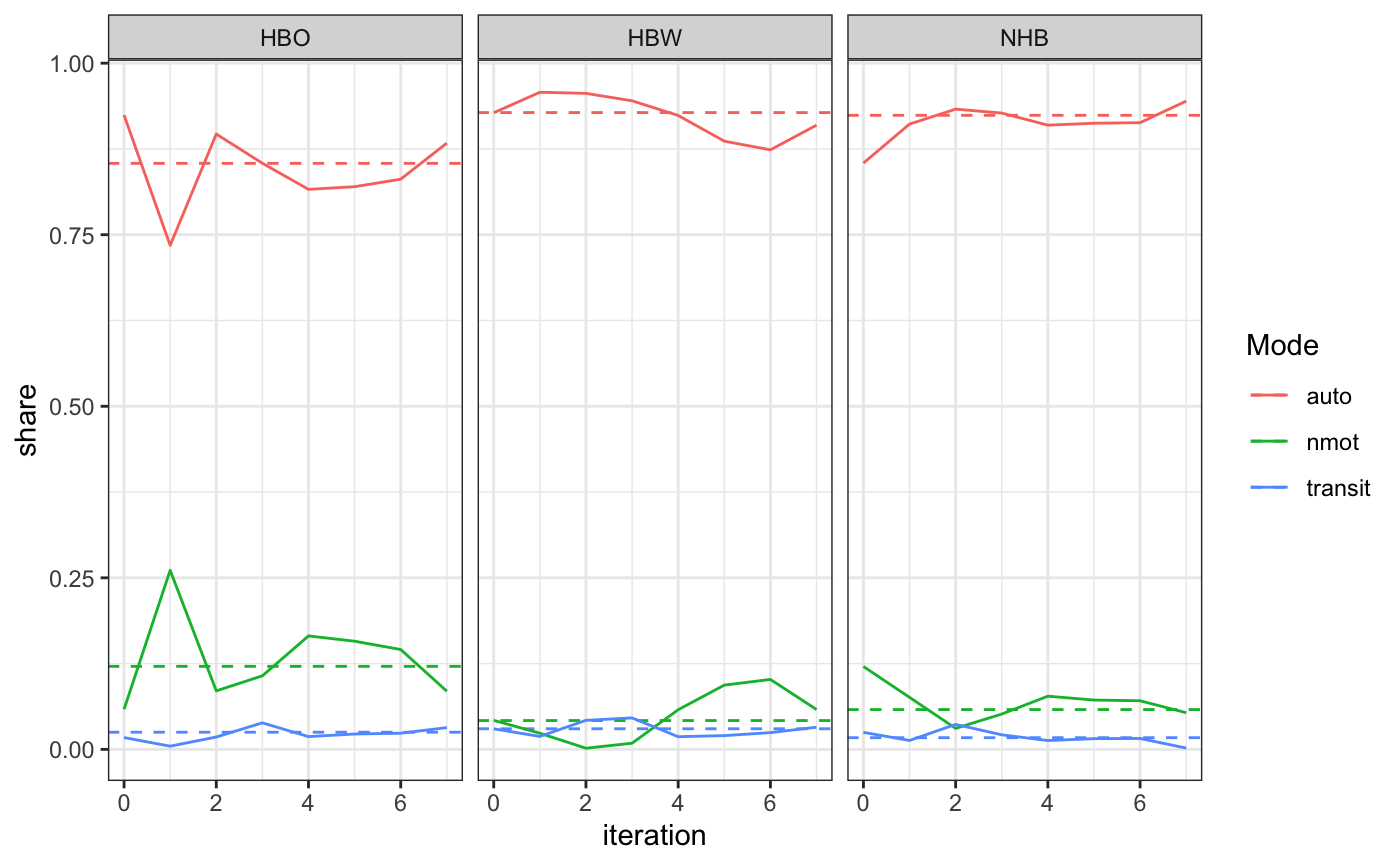
\includegraphics[width=0.75\linewidth]{figures/chapter3/MC_split.png}

  }

  \caption{Mode choice splits by trip purpose.}\label{fig:nhbmc}
  \end{figure}

The DC parameters were also calibrated, however this process differed slightly
from the MC constant calibration process. A destination choice model is also a
multinomial logit model, but this model cannot have alternative-specific
constants because of the high numbers of alternatives (one alternative for
every zone). Instead, the destination choice utility equation can include a
calibration polynomial that adjusts the implied utility to match a trip length
frequency distribution (TLFD) extracted from USTM. In this model, a
cubic polynomial  is included as the destination choice calibration term seen below:
\begin{equation}
  f(d_{ij}) = \kappa_1 d_{ij} + \kappa_2 d_{ij}^2 + \kappa_3 d_{ij}^3
	\label{eqn:poly}
\end{equation}

\noindent where $d_{ij}$ represents the distance from $i$ to $j$
and each of the  '$\kappa_1,\kappa_2,\kappa_3$, are calibrated to minimize the
difference between the model and target trip length frequency distribution. The target
values for calibration are derived from USTM. The cubic polynomial in
Equation \ref{eqn:poly} --- which is part of the DC utility in
Equation \ref{eqn:dc} --- was applied and calibrated to match the target TLFD
values from USTM. The final calibration values are presented in Table
\ref{tab:coeffs}.

\subsection{Calibration Results}

To ensure that calibration efforts were successful, it was necessary to
compare the TLFD results from USTM and the Resiliency Model. A
TLFD script that could divide trips
into distance bins was created. Dividing the trips into distance bins allows for the
breakdown of resiliency trip frequencies by destination, which can then be
compared to the original USTM values. Initial target values for total
trips by purpose were extracted from USTM to ensure that trips in
the Resiliency Model were being conserved. Trip totals were compared using
the TLFD outputs to ensure trips of similar lengths were being estimated,
and to the total trips by purpose and mode to ensure trip conservation.

Final trip length distributions for each purpose are similar to the
extracted USTM target values for both the TLFD comparison and the overall
total value comparison. Additionally, Figure \ref{fig:ustm_tlfd} shows the original versus the final
TLFD for the USTM and resilience models. The fit for both is similar, though
there is some variation present between each trip purpose considered.

\begin{figure}

{\centering 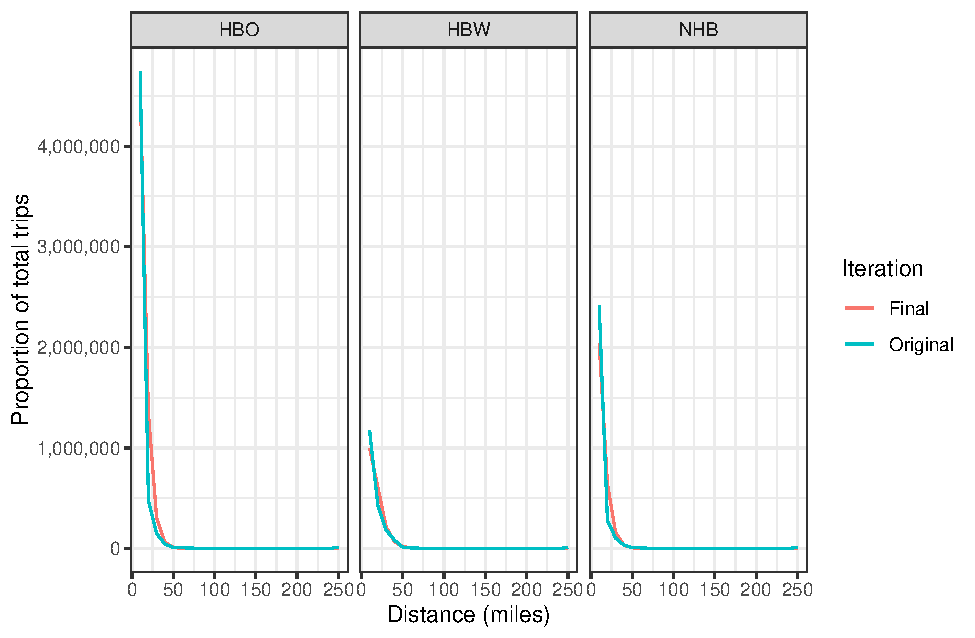
\includegraphics[width=0.75\linewidth]{figures/chapter3/TLFD.pdf}

}

\caption{Original and final trip length frequency distribution.}\label{fig:ustm_tlfd}
\end{figure}


\section{Method to Calculate Costs for Non-model Purposes}

Some trip purposes contained in USTM did not have enough available data to
include in the logsum portion of the Resiliency Model or did not have
significant impacts and were left out of the logit-based model
calculation. This section will discuss other methods by which costs
associated with each link could be calculated, especially for those
purposes not primarily included in the Resiliency Model and for comparison purposes.

Purposes including freight, recreation (REC), and home-based college
(HBC) trips were evaluated using overall travel time change. These
purposes are either rigid in their origins and destinations, as is the
case with most freight trips, or have much smaller frequencies than do the
three main trip purposes HBW, HBO, NHB included in the Resiliency
Model. At the same time, the data needed to create logsum calculations for these
excluded purposes was not readily available. As a result, the costs associated with these trip
purposes was computed based on the increase, or change, in travel time between the base
scenario and an alternative scenario.

The travel time difference is calculated by comparing the change in travel
time between the base scenario and any alternative scenario. The base
scenario highway skim module chooses a route between an OD pair based on
the shortest travel time, not the shortest distance. Thus, the difference
in travel times always remained the same, or increased. The distances, however,
could become shorter, as the shortest distance between an OD pair was not
always the fastest by time. Equation \ref{eqn:time} shows a representation of how
differences in travel time were calculated:
\begin{equation}
	\Delta tt_{ij} = ScenarioTime_{ij} - BaseTime_{ij}
	\label{eqn:time}
\end{equation}

Finding the difference in travel time for each scenario allows for
additional costs to be incorporated that are not included in the logsum
calculation performed on the HBW, HBO, and NHB purposes.

Applying a VOT evaluation, the cost associated with link
closure per day can be measured for each of the purposes not included in
the main logsum analysis. Freight trips and auto trips have different
values of time in USTM, thus the calculated travel time change was
multiplied by different VOTs for each purpose. For passenger vehicle
trips, a VOT of \$17.67 was used, while for freight trips, a VOT of
\$94.04 per hour was used. These values were extracted from USTM and
verified by UDOT's Asset Risk Management Guide \citep{UtahDepartmentofTransportation2020}.
Additionally, the VOT for the logsum method equates to \$16.87 per hour as seen in
Table \ref{tab:VOT}

\begin{table}


\caption{\label{tab:VOT}Values of Time for Time Difference Calculations}
\centering
\begin{tabular}[t]{cccl}
\toprule
Freight & Auto & Logsum\\
\midrule
94.04 & 17.67 & 16.87 & Dollars/Hr\\
156.73 & 29.45 & 28.11 & Cents/Min\\
\bottomrule
\end{tabular}
\end{table}

The conversion between the measured DCLS and the actual cost for the logsum method differs from the conversion for the travel time method.
In Table \ref{tab:coeffs}, the coefficient \(\beta_{cost}\) is equal to -0.0016.
To convert between the change in DCLS, or dis-benefit, and the monetary cost to a
single user for each purpose, the following equations must be used:
\begin{equation}
  \Delta{Logsum_{im}} = \frac{-1}{\beta_{cost m}} *(DCLS^{Base}_{im} - DCLS^{Scenario}_{im})
\end{equation}
then, for all trips starting at \(i\), the total benefit is:
\begin{equation}
  \Delta{Logsum_{im}} * P_{im}
\end{equation}
This gives an estimate of the cost experienced by the whole network as a result
of the closure of a single link.

\section{Summary}

The creation of a logit-based model, which is sensitive to mode and destination
choice, allows for more sensitive and robust estimations of accessibility because
of the ease with which additional data types can be incorporated into the model. The
model also accounts for modes that are not flexible in the case of link
closure. The Resiliency Model is capable of analyzing the effects of
road closure on mode and destination choice, and it can estimate overall
dis-benefit (in dollars) experienced by road users per day.
